% -*- Mode:TeX -*-

%% IMPORTANT: The official thesis specifications are available at:
%%            http://libraries.mit.edu/archives/thesis-specs/
%%
%%            Please verify your thesis' formatting and copyright
%%            assignment before submission.  If you notice any
%%            discrepancies between these templates and the 
%%            MIT Libraries' specs, please let us know
%%            by e-mailing thesis@mit.edu

%% The documentclass options along with the pagestyle can be used to generate
%% a technical report, a draft copy, or a regular thesis.  You may need to
%% re-specify the pagestyle after you \include  cover.tex.  For more
%% information, see the first few lines of mitthesis.cls. 

%\documentclass[12pt,vi,twoside]{mitthesis}
%%
%%  If you want your thesis copyright to you instead of MIT, use the
%%  ``vi'' option, as above.
%%
%\documentclass[12pt,twoside,leftblank]{mitthesis}
%%
%% If you want blank pages before new chapters to be labelled ``This
%% Page Intentionally Left Blank'', use the ``leftblank'' option, as
%% above. 

\documentclass[11pt,oneside]{mitthesis}
\usepackage{lgrind}
\usepackage{titlesec}
\usepackage{pgfplots}
\usepackage{listings}
\usepackage{pdfpages}
\lstset{language=C}
\usepackage{nomencl}


\usepackage[europeanresistors]{circuitikz}

\usepackage{tikz}
%% These have been added at the request of the MIT Libraries, because
%% some PDF conversions mess up the ligatures.  -LB, 1/22/2014
\usepackage{cmap}
\usepackage[T1]{fontenc}
\usepackage[utf8]{inputenc}
\pgfplotsset{every axis legend/.append style={
at={(1.1,0.2)},
anchor=south west}} 


\pagestyle{plain}
\titlespacing\section{0pt}{12pt plus 4pt minus 2pt}{12pt plus 4pt minus 8pt}
\renewcommand{\chaptername}{Kapitola}
\renewcommand{\figurename}{Obrázek}
\renewcommand{\tablename}{Tabulka}
\renewcommand{\contentsname}{Obsah}
\renewcommand{\contentsname}{Obsah}
\renewcommand{\listtablename}{Tabulky}
\renewcommand{\listfigurename}{Obrázky}

%\addtocontents{toc}{\protect\thispagestyle{empty}}
%\addtocontents{lof}{\protect\thispagestyle{empty}}

\newcommand{\itab}[1]{\hspace{0em}\rlap{#1}}
\newcommand{\tab}[1]{\hspace{.2\textwidth}\rlap{#1}}

\newcommand\uv[1]{\quotedblbase #1\textquotedblleft}
\usepgfplotslibrary{polar}
\makenomenclature

\begin{document}

\include{cover}


\pagestyle{plain}
\include{contents}

\setcounter{page}{1}
%% This is an example first chapter.  You should put chapter/appendix that you
%% write into a separate file, and add a line \include{yourfilename} to
%% main.tex, where `yourfilename.tex' is the name of the chapter/appendix file.
%% You can process specific files by typing their names in at the 
%% \files=
%% prompt when you run the file main.tex through LaTeX.
\chapter{Úvod}
Téma anténních struktur osazených čočkami, zejména anténních čoček jako takových, bylo vemi aktuální a rozvíjené v počátcích vývoje antén pro mikrovlnnou techniku. Avšak s příchodem reflektorových antén se velká část pozornosti odklonila právě k nim zejména z důvodu jejich vyšší efektivity. Poslední dobou se stále se zvyšujícím kmitočtem, anténní struktury s čočkami začínají opět získávát svoji poroznost. \cite{ModernLens}

\section{Motivace}
3D tisk je technologie zejména pro výrobu rychlých prototypů, takzvaný "rapid prototyping", používaná ve stále více oborech. S uvedením speciálních polymerních materiálů vykazující vyšší elektrickou vodivost do prodeje má stále větší smysl využití právě této technologie pro urychlení vývoje a malosériovou výrobu antén (s vyjímkou dielektrických rezonančních struktur).

\section{Cíl}
Primárním cílem této práce je výzkum využití 3D tiskové technologie FDM pro výrobu anténní struktury (trychtýřová anténa s dielektrickou čočkou) od návrhu optimalizovaného pro jednoduchou výrobu, přez extrakci dielektrických parametrů po průchodu technologickým procesem, po vlastní realizaci navržené struktury na frekvenci 10\,GHz. Sekundárním cílem práce byl průzkum možností následného pokovení pro minimalizaci rozdílu mezi "vytisknutou" a profesionálně realizovanou strukturou.
%% This is an example first chapter.  You should put chapter/appendix that you
%% write into a separate file, and add a line \include{yourfilename} to
%% main.tex, where `yourfilename.tex' is the name of the chapter/appendix file.
%% You can process specific files by typing their names in at the 
%% \files=
%% prompt when you run the file main.tex through LaTeX.
\chapter{Teoretický rozbor}
Před vlastním návrhem a realizací je nezbytně nutné být seznámen alespoň se základní teorií použitých technologií a postupů. Bez této znalosti by se jednalo pouze o útržky textu a nebylo by možno zacházet do řešení komplexnější problematiky a kladení možných dalších témat pro následující výzkum a posun technologie.

\section{3D tisk a materiály}
3D tisk je na rozdíl od jiných technologií aditivní proces. Jedná se tedy o postupné přidávání základního materiálu v diskrétních krocích (vrstvách).
Technologií existuje několik a s postupným rozšiřováním možností aplikace jich stále přibývá. Pro řešení této práce byla vybrána technologie FDM vzhledem k jejímu masovému rozšíření, dostupnosti a nízkých nákladů. 

\subsection{Princip technologie FDM}
Fused deposition modeling, zkráceně FDM, případně FFF (Fused Filament Fabrication) je technologie 3D tisku využívající možnost opakovatelného přechodu mezi skupenstvími působením energie ve formě tepla termoplastických polymerních materiálů. Základní materiál ve formě filamentu (drátu) definovaného průměru, zpravidla 1.75\,mm, nebo 2.85\,mm, je vtlačován do předehřáte trysky silou $F$. Pokud teplota horké zóny trysky převyšuje teplotu skelného přechodu vtlačovaného materiálu dojde k dramatickému oslabení mezimolekulárních sil a vzniku viskózní kapaliny. Jelikož je průměr trysky velmi blízký průměru vtlačovaného filamentu, s vyjímkou jejího hrdla které je násobně menší, zpravidla 0.4\,mm, jediná možnost jak uvolnit vnitřní tlak je vytlačení kapaliny hrdlem. Jakmile teplota vytlačené kapaliny klesne pod teplotu skelného přechodu dojde k obnovení mezimolekulárních sil a materiál je opět pevnou látkou. Tento jev je obecně znám pod názvem extruze.
Toto nám však nestačí pro vytvoření trojrozměrného objektu dle zadání. Je tedy třeba extrudér osadit na zařízení zajišťující pohyb v trojrozměrném prostoru.
Proces tisku pak probíhá pohybem extrudéru po předem definovaných trasách, zpravidla vždy v jedné vrstvě, a vytlačováním materiálu dle potřeby. Celý proces se poté opakuje dokud není dokončen zadaný objekt.
\begin{figure}[h]
\begin{center}
\includegraphics[width=7.5cm]{pics/fdm}
\caption{Princip technologie FDM. 1 - Tisková podložka, 2 - Již hotové vrstvy výsledného objektu, 3 - Horká zóna trysky, 4 - Tryska, 5 - Filament, F - Vtlačovací síla}
\end{center}
\end{figure}


\subsection{Vlastnosti technologie}
3D tisk, podobně jako jiné technologie má specifické vlastnosti, které ovlivňují charakter výsledného produktu. Ovlivněných vlastnostností je velmi mnoho, pro naši aplikaci se zaměříme na dielektrické (chceme vědět jaké bude mít výsledný produkt dielektrické vlastnosti, abychom ho byly schopni popsat, navrhovat a simulovat) a mechanické (produkt musí být možno pevně a stabilě ukotvit na pozici, a musí do něj být možno navázat elektromagnetickou vlnu známým způsobem). Je však nutno brát v potaz, že má i celou řadu vlastností, kterých lze využít pro vytvoření složitých struktur, které by nebylo možné jinými technologiemi jednoduše realizovat, například vnitřní uzavřené struktury. Některé z nich jsou zatím pro dostatečně přesné aproximace dosažitelné v reálném časovém horizontu zcela náhodné, jiné zase přímo ovlivňují námi velmi žádané parametry a můžeme je takto řídit.
\subsubsection{Vrstvy}
Pokud budeme uvažovat ideální podmínky (absolutně čisté prostředí bez kontaminace nechtěnými látkami, ideální filament, rovnoměrnou kontrolovanou distribuci tepla, atd...) stále je objekt tvořem z vrstev. Jelikož vždy vrtva, na které se aktuálně nanáší, je dokonce pod teplotou skelného přechodu, pro odstranění deformace vlivem sil jako gravitace, či tepelné roztažnosti, nedojde k dokonalému spojení polymerních řetězců mezi vrtvami. Při laminaci vrstev může také dojít ke kontaminaci produktu, jako například prachovými částicemi či vzduchovými kapsami. Toto se však dá zanedbat jelikož lze snadno stabilizovat okolní prostředí a minimalizovat vliv. 
Hlavní ovlivněné vlastnosti, pro naši aplikaci podstatné, jsou mechanické. Vždy je v ose vrstev rozložení mezne plasticity neuniformní, dochází tedy k plastické deformaci významně v těchto oblastech, což někdy může být problém z důvodu nutnosti splnění možnosti upevnění a realizovatelnosti produktu.
Z dielektrického hlediska tedy nebude ani relativní permitivita uniformně rozložená v jedné ose, vznikne tedy periodická stuktura. Tento vliv by bylo možné omezit buďto zvýšením diskretizačního kroku, tedy omezením počtu rozhraní, což může v jistých případech ovlivňovat vlastnosti celé struktury vzhledem růstu kvantizačního šumu, nebo naopak snížením kroku kdy již bude úroveň šumu blízká nule, což se bohužel negativně projeví na době tisku, to však v některých případech není problém. Výzkum popisu tohoto chování je však předmětem dalším.

\subsubsection{Vnitřní struktury}
Vlivem principu vrstvení je možno vytvářet vnitřní struktury definovaných tvarů, dokonce i selektivně, a takto velmi silně ovlivňovat pro nás důležité parametry.
Mechanické vlastnosti tímto lze slektivně měnit, například zpevněním montážních ovorů v technologickém okolí, což v našem případě není první v pořadí.
Dielektrické vlastnosti jsou tímto však velmi ovlivněny. Technologií je totiž možno vytvářet prakticky jakékoliv struktury uvnitř produktu ve zvolených místech, tedy například vytisknout Luneburgovu či Maxwell fish-eye čočku. Je však ale nutno provést výzkum na toto téma dostatečné podrobrý výzkum, jedná se totiž o skokové změny vlastností. Tyto změny poté vytváří rozhraní, kde dochází odrazům, které zatím modelovat a popsat je velmi komplexní úlohou.

\begin{figure}[h]
\begin{center}
\includegraphics[width=8.5cm]{pics/fillcompare}
\caption{Porovnání různého motivu vrstvy, a) 100\,\% vyplň typem rectilinear, b) 20\,\% vyplnň typem cubic}
\end{center}
\end{figure}

\begin{figure}[h]
\begin{center}
\includegraphics[width=8.5cm]{pics/6layer}
\caption{Náhled vrstev 1-6 struktury s kombinovanou výplní typu rectilinear (první dvě vrstvy) a cubic o rozdílné procentuální výplni}
\end{center}
\end{figure}

\subsection{Materiály využitelné pro vysokofrekvenční techniku}
Termopolymerních materiálů které by se daly využít je celá řada, teoreticky je možné uplatnit velké množství, prakticky však ale vyplývá otázka bezpečnosti, jelikož průchod některých polymerů procesem může uvolňovat nebezpečné látky, či v případě směsí její části. Dále je však nutné brát v potaz i vlastnosti jako tepelná roztažnost 
Mezi nejrozšířenější patří PLA, ABS a PET, tyto materiály však lze uplatnit zejména v čočkách, či dielektrických rezonátorech, jelikož vykazují velmi malou vodivost. Objevují se ale stále nové směsy materiálů jako například PLA s výraznou příměsí grafénových šupin, či měděného prachu které v ideálním případě disponují velmi vysokou vodivostí.

\subsubsection{"Vodivé" materiály}
Jelikož mezi nejrozšířenější materiály patří PLA, které vykazuje výborné zpracovatelské vlastnosti je většina těchno směsí právě na tomto nosiči.
Jako příměs pro vodivé materiály je možno použít teoreticky jakékoliv fragmenty vodivé látky jako třeba měď, stále populárnější je ale grafén, z důvodu jeho vysoké vodivosti způsobené $\pi$ elektrony. Při plnění nosného polymeru je však nutno brát v potaz že při zvyšujícím se podílu plniva se vlastnosti výsledné směsi velmi mění.
Jelikož je pro nás nyní nejvýznamnější elektrická vodivost, je tedy logický cíl maximalizace právě tohoto kritéria. Bohužel se ale stále bude jednat o směs vysoce vodivého materiálu ve velmi nevodivém polymeru, což má dramatický dopad na výsledek. V první řadě ikdyž budeme uvažovat dokonale uniformní rozložení a identické frakce příměsi ve filamentu, vlivem průchodu extrudérem nelze předpokládat, že výsledek bude stejný. Dochází totiž k opětovnému promísení a dokonalý popis celého systému zatím není znám. V druhé řadě je třeba stále brát ohled na zpracovatelnost materiálu a volit správné poměry příměsí, z pravidla 40 - 80\,\%[2- Konzultace Josef Doleček - Filamentum]. Z výše uvedených faktů je bohužel patrné, že výsledný produkt má nezanedbatelné dielektrické vlastnosti.
Ačkoliv se může zdát že tyto materiály nejsou pro naši aplikaci zatím použitelné, stále existuje možnost následného pokovení produktu, kde tyto vlastnosti výrazně zjednoduší proces.

\section{Trychtýřová anténa}
Trychtýřová anténa patří mezi základní anténní struktury využívané jak samostatně, tak ve formě ozařovačů reflektorových antén, či v kombinaci s anténní čočkou. Těchto struktur existuje několik druhů, v našem případě se ale zaměříme na nejpoužívanější, tedy pyramidální trychtýřovou anténu.
Tento typ antény byl zvolen zejména kvůli své jednoduchosti a požadavkům na technologii výroby.

\subsection{Základní princip}
Trychtýřová antená není nic jiného, než postupně se rozšiřující ústí vlnovodu v daných směrech. V případě pyramidálního trychtýře dochází k otevření jak v $E$, tak $H$ rovině. Postupné otevření trychtýře lze považovat za impedanční transformátor zajišťující, v ideálním případě bezodrazné, vyvázání vlny do volného prostoru v definovaném pásmu.
Základní parametry jsou vyobrazeny na obrázku \ref{fig:horn},\ref{fig:hornEH}.

\begin{figure}[h]
\begin{center}
\includegraphics[width=9.5cm]{pics/horn}
\caption{Pyramidální trychtýřová anténa}
\label{fig:horn}
\end{center}
\end{figure}

\begin{figure}[h]
\begin{center}
\includegraphics[width=15cm]{pics/hornEH}
\caption{Pyramidální trychtýřová anténa v řezu a)E-roviny, b)H-roviny}
\label{fig:hornEH}
\end{center}
\end{figure}
\begin{itemize}
\item $a, b$ - Rozměry vlnovodu
\item $a_1, b_1$ - Rozměry ústí trychtýře
\item $x', y'$ - E-rovina, H-rovina
\item $z'$ - Směr Poyntingova vektoru
\item $\rho$ - Délka stěny trychtýře
\item $p$ - Délka trychtýře
\item $\psi$ - Úhel otevření
\end{itemize}

\subsection{Charakterizace struktury}


\subsubsection{Směrovost a zisk}
Směrovost charakterizuje strukturu z hlediska poměru intenzit vyzářeného výkonu struktury do určitého směru, ku celkovému vyzářenému výkonu do celého prostoru. Jde tedy o schopnost antény "směrovat" výkon do určitého směru. Toto však z principu reciprocity paltí i opačně, tedy pro přijatý výkon. Na základě tohoto lze definovat maximální směrovost antény.

\renewcommand{\figurename}{}
\begin{center}
\LARGE{$G_p/dB = 10*[1.008+\log_{10}(\frac{a_1 * b_1}{\lambda^2})]$}
\begin{figure}[h]
\caption{Maximální směrovost pyramidální trychtýřové antény}
\label{fig:hornG}
\end{figure}
\end{center}
\renewcommand{\figurename}{Obrázek}

\renewcommand{\figurename}{Obrázek}
Zisk antény je však pro aplikace zajímavějším parametrem, jelikož zahrnuje i ztráty vyzařovací účinností $\eta_r$.
\renewcommand{\figurename}{}
\begin{center}
\LARGE{$G_{dB} = D_{dB} - \eta_{r(dB)}$}
\begin{figure}[h]
\caption{Vztah zisku a směrovosti}
\label{fig:hornG}
\end{figure}
\end{center}
\renewcommand{\figurename}{Obrázek}

\subsubsection{Fázová chyba}
Jelikož při vyvazování vlny z vlnovodu do volného prostředí dochází k transformaci vlny rovinné na kulovou. Z této skutečnosti plyne, že na rozhraní ústí trychtýře bude existovat oblast, kde se střed vlny bude nacházet právě na rozhraní, ale její okraje stále uvnitř. Tento rozdíl se nazývá fázová chyba a vede k deformaci směrové charakteristiky a snížení směrovosti. Pro minimalizaci této chyby je vhodné, aby úhel otevření trychtýře byl co nejmenší, nicméně je však ale nutno brát v potaz, že tímto narůstá jeho odélka a zároveň i náročnost realizace.
\begin{figure}[h]
\begin{center}
\includegraphics[width=6.5cm]{pics/hornErr}
\caption{Znázornění fázové chyby $Y$}
\label{fig:HornErr}
\end{center}
\end{figure}


\newpage
\section{Anténní čočky}
Podobně jako v optice, i zde lze použít čočku, jelikož světlo má z důvodu duality i charakter vlny. Existuje tedy celá řada různých realizací čoček, lze je rozdělit do dvou základních kategorií:
\begin{itemize}
\item Zpomalovací, neboli dielektrické
\item Urychlující, neboli kovové
\end{itemize}

\subsection{Základní princip}
Hlavním úkolem čočky je kolimovat paprsek, neboli šnížit rozbíhavost, v případě anténní domény transformovat kulovou vlnu na rovinnou. Jak můžeme vidět na obrázku \ref{fig:hornLens}, kde:
\begin{itemize}
\item $1$ - Trychtýřová anténa
\item $2$ - Vystupující kulová vlna z trychtýře
\item $3$ - Anténní čočka
\item $4$ - Výsledná rovinná vlna
\item $X$ - Parametr kulovitosti vstupní vlny
\item $X'$ - Parametr kulovitosti výstupní vlny
\end{itemize}
\begin{figure}[h]
\begin{center}
\includegraphics[width=9.5cm]{pics/lens}
\caption{Princip anténní čočky}
\label{fig:hornLens}
\end{center}
\end{figure}
Pro zajištění této funkce je však ale nutno, aby anténní čočka měla rozdílnou relativní permitivitu $\epsilon_r$ než okolní prostředí, ve kterém se vlna šíří. Touto podmínkou je způsobeno zpomalení, nebo zrychlení, vlny a následné kolimaci. Z čehož plyne již výše uvedené rozdělení čoček, viz obrázek \ref{fig:LensTypes}.
\begin{figure}[h]
\begin{center}
\includegraphics[width=9.5cm]{pics/lenstypes}
\caption{Typy anténních čoček. 1 - Zpomalující, 2 - Zrychlující}
\label{fig:LensTypes}
\end{center}
\end{figure}

\section{Extrakce dielektrických parametrů}
Znalost dielektrických parametrů je klíčová pro návrh vlastních strukur, zejména anténních čoček.
Pro většinu materiálů jsou tyto parametry již známé, nicméně pokud se rozhodneme strukturu realizovat technologií 3D tisků, vstypuje do tohoto mnoho dalších proměnných které mohou výrazně ovlivnit výsledné parametry produktu, ať už v prospěch, či naopak.
Pro získání těchto parametrů lze použít například proces integrovaný v CST MW studio, který lze papsat blokovým schématem na obrázku \ref{fig:ExtractBlock}
\begin{figure}[h]
\begin{center}
\includegraphics[width=9.5cm]{pics/ExtractBlock}
\caption{Blokové schéma extrakce dielektrických parametrů}
\label{fig:ExtractBlock}
\end{center}
\end{figure}
\subsection{Princip extrakce}
Extrakce parametrů spočívá ve změření přenosu mezi kanály $A$ a $B$ vektorového analyzátoru pro dva geometricky odlišné vzorky materiálu, jehož parametry chceme extrahovat. Jelikož v systému dojde ke změně pouze rozměru neznámého materiálu, tak na základě rozdílného přenosu jsme schopni z naměřených dat extrahovat dielektrické parametry jako relativní permitivitu $\epsilon_r$ a ztrátový činitel $tg_\delta$.

%% This is an example first chapter.  You should put chapter/appendix that you
%% write into a separate file, and add a line \include{yourfilename} to
%% main.tex, where `yourfilename.tex' is the name of the chapter/appendix file.
%% You can process specific files by typing their names in at the 
%% \files=
%% prompt when you run the file main.tex through LaTeX.
\chapter{Návrh}
Hlavním cílem této práce je realizace anténní struktury pomocí technologii 3D tisku, a jelikož jako kterýkoliv jiný technologický proces má své omezení vyplívající z jeho principu, je vhodné tyto charakteristické vlastnosti brát v potaz již při návrhu.

Pokud se toto dodří, minimalizuje se dopad nedokonalostí technologie, výrazně se zjednoduší realizace a splnění podmínky minimální post produkce produktu před jeho možným použitím.

\section{Trychtýřová anténa}
K návrhu trychtýřové antény lze přistoupit řadou různých způsobů, od odvození, přez aplikaci návrhových vzorů, až po využití moderních podpůrných software řešení typu Antenna magus. Jelikož tato práce je zaměřena zejména na výzkum možnosti uplatnění technologie 3D tisku pro výrobu této anténní struktury, byla zvolena cesta návrhu za podpory software Antena magus.

Zvolené řešení umožnilo vyloučení návrhových chyb v porovnání s komplexními cestami a poskytlo optimální prvotní návrh, na kterém pak byly provedeny úpravy pro minimalizaci vlivů použité technologie. Další velmi významnou výhodou bylo poskytnutí plně parametrického modelu, což znamenalo znatelnou časovou úsporu, jak při návrhu, tak následné optimalizaci modelu.
\subsubsection{Vstupní model antény}
Geometrické rozměry optimálního trychtýře jsou následující:
\begin{itemize}
\item $a_1 = 110\,mm$ - Šířka ústí
\item $b_1 = 79\,mm$ - Výška ústí
\item $p = 228\,mm$ - Délka trychtýře
\item $plth = 0.15\,mm$ - Tloušťka stěny
\end{itemize}

\begin{figure}[h]
\begin{center}
\includegraphics[width=9.5cm]{pics/HornOptimal}
\caption{Vstupní model antény}
\label{fig:hornOptimal}
\end{center}
\end{figure}

Jelikož ale standartně dostupné 3D tiskárny disponují pouze maximální možnou výškou výsledného produktu 200\,mm a průměrem trysky 0.4\,mm je patrné, že je třeba návrh struktury mírně zoptimalizovat.

Prvním parametrem, který je třeba změnit je délka trychtýře $p$. Je ale však nutné brát v potaz, že tento parametr je pouze délka samotného trychtýře. Jelikož ale potřebujeme i úsek vlnovodu, aby se střed trychtýře nacházel ve stejném prostředí, z důvodu stabilních podmínek, a samozřejmě bychom rádi strukturu osadili na vlvnovod, musíme počítat s rezervou a nelze tedy nastavit  $p=200\,mm$.

Druhým parametrem je poté samozřejmě tloušťka stěny $plth$, která při hodnotě 0.15\,mm bude nerealizovatelná, jelikož je několikanásobně menší, než průměr vlastní trysky. Podobně jako u předchozího případu musíme počítat s rezervou, tentokrát však je ale podmínka více obnecná. Pro udržení mechanické pevnosti struktur z důvodu chladnutí v průběhu procesu platí pravidlo alespoň dvojnásobné šířky extruze, tedy dle \ref{eq:MinWidth} (kde reprezentuje $W_{MIN}/mm$ minimální šířku stěny v mm a $D_{nozzle(mm)}$ průměr trysky v mm) minimum $plth = 0.9\,mm$

\begin{equation}
W_{MIN}/mm = 2*(D_{nozzle(mm)}+0.05)
\label{eq:MinWidth}
\end{equation}

\subsubsection{Optimalizovaný model antény}
Po přiblížení se k výše uvedených optimalizačních cílů dostaneme následující parametry struktury:
\begin{itemize}
\item $a_1 = 110\,mm$ - Šířka ústí
\item $b_1 = 79\,mm$ - Výška ústí
\item $p = 140\,mm$ - Délka trychtýře
\item $plth = 1.45\,mm$ - Tloušťka stěny
\end{itemize}
Zde však nebyla volba zejména $plth = 1.45\,mm$ zcela optimální, aby bylo by možné v případě komplikací při procesu použít například $D_{nozzle} = 0.6\,mm$ 

Kde poté na srovnání \ref{fig:hornCompare} jsou viditelné nepatrné rozdíly pouze zkráceného (A), zkráceného s realizovatelnou šířkou stěny (B), včetně skutečně optimální (C) a zkráceného s realizovatelnou šířkou stěny a zavedenou udávanou vodivostí plánovaného materiálu na realizaci (D) trychtýře. Samotný vliv zkrácení trychtýře je již uveden na \ref{fig:HornLenDep}.

\begin{figure}
\begin{tikzpicture}[scale=1.4]
\begin{axis}[
    xlabel={Angle /\,$^\circ$},
    ylabel={Amplitude /\,dB},
    minor tick num=10,
    minor grid style={gray!25},
  	major grid style={black!50},
  	xmin=-180,xmax = 180,
  	%ymin=-120, ymax=-60,
    grid=both
]
\addplot [no markers, thick, blue] table [col sep=tab, y=Ae140thin] {hornSim.dat};
\addplot [no markers, thick, green] table [col sep=tab, y=Ae140thick] {hornSim.dat};
\addplot [no markers, thick, red] table [col sep=tab, y=Ae140thickOpt] {hornSim.dat};
\addplot [no markers, thick, orange] table [col sep=tab, y=Ae140thCond] {hornSim.dat};
\legend{A,B,C,D};
\end{axis}
\end{tikzpicture}
\caption{Řezy směrových charakteristiky v E rovině, kde: \textbf{A}-$p=140\,mm$, \textbf{B}-$p=140\,mm$; $plth=1.45\,mm$, \textbf{C}-$p=140\,mm$; $plth=0.9\,mm$, \textbf{D}-$p=140\,mm$; $plth=1.45\,mm$; $G=133.3\,S/m$}
\label{fig:hornCompare}
\end{figure}

\begin{figure}[h]
\begin{center}
\includegraphics[width=9.5cm]{pics/HornFinal}
\caption{Výsledný model trychtýřové antény včetně příruby na vlnovod}
\label{fig:HornFinal}
\end{center}
\end{figure}

\subsubsection{Optimalizovaný model antény pro možnost post-produkce}
Uvažujeme-li aktuální reálné parametry, vliv technologie realizace a další proměnné, je velmi pravděpodobné, že pro praktické použití nebudé smysluplné. Nicméně mohou postačovat pro následnou post-produkci, která při použití standartních materiálů je velmi komplikovaná, jako například pokovení.

Budeme-li chtít navrhnout strukturu pro tento postup, musíme model optimalizovat dále, jelikož i technologie následného pokovení má svá úskalí, jako například obtížné pokovení uvnitř dutin, vlnovodů. Zejména obtížné pokovování dutin je velmi význámné omezení, pokud naše struktura je právě trychtýř a stejnoměrné pokovení uvnitř je zásadní.

Toto však snadno opet využitím technologie 3D tisku snadno vyřešit, v porovnání s úpravou pokovovacího procesu (nikoliv jeho parametrů). Tedy řezem středu trychtýře v E rovině, pro minimální ovlivnění povrchových proudů vnější stranou trychtýře a lehkého potlačení zadního laloku \ref{fig:hornCompareAssy}, a po následném pokovení mechanickým spojem. 

\begin{figure}[h]
\begin{center}
\includegraphics[width=9.5cm]{pics/HornAssy}
\caption{Výsledný model trychtýřové antény včetně příruby na vlnovod a následné sestavení}
\label{fig:HornAssy}
\end{center}
\end{figure}

\begin{figure}
\begin{tikzpicture}[scale=1.4]
\begin{axis}[
    xlabel={Angle /\,$^\circ$},
    ylabel={Amplitude /\,dB},
    minor tick num=10,
    minor grid style={gray!25},
  	major grid style={black!50},
  	xmin=-180,xmax = 180,
  	%ymin=-120, ymax=-60,
    grid=both
]
\addplot [no markers, thick, blue] table [col sep=tab, y=Ae140thickPrir] {hornSim.dat};
\addplot [no markers, thick, green] table [col sep=tab, y=Ae140thickAssy] {hornSim.dat};
\legend{A,B};
\end{axis}
\end{tikzpicture}
\caption{Řezy směrových charakteristiky v E rovině, kde: \textbf{A} - Původní optimalizovaný trychtýř, \textbf{B} - Trychtýř s přírubami na sestavení}
\label{fig:hornCompareAssy}
\end{figure}

\section{Extrakce dielektrických parametrů}
Jak již víme, metod extrakce dielektrických parametrů, zejména komplexní permitivity a ztrátového činitele, existuje velmi mnoho. Pro účely této práce byla zvolena transmisní/reflexní metoda, která je velmi vhodná, zejména při použití ve vlnovodu, pro realizaci použitou technologií.

Abychom zajistili následnou možnost použití extrahovaných parametrů, zejména pro návrh anténní čočky, je nezbytné materiál charakterizovat v použitém kmitočtu, tedy 10\,GHz.

Na základě definovaného kmitočtu a použité metody je nutno navrhnout výplně vlnovodu, které budou následně podrobeny měření \ref{fig:ExtractBlock}. Pro přesnou extrakci parametrů je velmi důležité zachovat celkovou délku systému $L$ a udržení měřeného vzorku ve středu pro minimalizaci fázové chyby, tedy v případě krašího vzorku symetricky doplnit úseky vlnovodu. Dalším důležitým parametrem pro extrakci přesných dat je vhodné, aby útlum měřených vzroků byl alespoň 3\,dB, od čehož se bude odvíjet celková délka vkládaných vzorků.

\begin{figure}[h]
\begin{center}
\includegraphics[width=9.5cm]{pics/ExtractBlock}
\caption{Blokové schéma transmisní/reflexní extrakce dielektrických parametrů}
\label{fig:ExtractBlock}
\end{center}
\end{figure} 




\section{Anténní čočka}
Na základě znalosti "vodivých" materiálů a jejich charakteru byl zvolen dielektrický typ čočky, konkrétně plano-konvexní čočka zejména kvůli vyšší předvídatelnosti chování dielektrických materiálů po průchodu technologickým procesem.
Jak již víme, k návrhu anténní čočky, lze přistupovat podobně jako k návrhu čočky optické.
Aby čočka splňovala svojí funkci transformace kulové vlny na rovinnou v dané aplikaci, je nutné zvolit pro následný návrh ohniskovou vzdálenost $F$ a průměr čočky $D$, které přímo lze spočítat na základě znalosti geometrických rozměrů antény.
Jako ohniskovou vzdálenost čočky je vždy nutné určit tak, aby zdroj byl právě v tomto bodě pro zajištění maximálně rovinné vlny. Rozhodneme-li se umístit čočku přímo na ústí struktury, musí být být ohnisková vzdálenost právě rovna $p_1$. Za použití základní geometrie lze odvodit vztah vztah \ref{eq:lensF}, kde poté vychází $F = 160\,mm$
\begin{equation}
F = p + \frac{\frac{b_1}{2}-(tg(\psi) p) }{tg(\psi)}
\label{eq:lensF}
\end{equation}
Jelikož je důležité, aby čočka zároveň překrývala celou plochu ústí trychtýře, a příliš nepřesahovala, z důvodu minimalizace časové náročnosti realizace a objemu materiálu, lze její průměr vypočítat ze vztahu \ref{eq:lensDia}, kde po dosazení vychází $D = 136\,mm$.
\begin{equation}
D = \sqrt{a_1^2+b_1^2} 
\label{eq:lensDia}
\end{equation}
Posledním nezbytným parametrem pro finální je poloměr zakřivení čočky $R$. Tento zbývající parametr lze na základě známého návrhového pravidla \ref{eq:lensRad}, kde $\epsilon_r-lens$ je relativní permitivita materiálu čočky a $\epsilon_r-space$ relativní permitivita prostředí, po dosazení, a samozřejmě předchozí exktrakce dielektrických parametrů materiálu, ze kterého bude následně čočka vytvořena, dospět k $R = 192\,mm$.
\begin{equation}
R = (\epsilon_{r-lens} - \epsilon_{r-space})F
\label{eq:lensRad}
\end{equation}

\begin{figure}[h]
\begin{center}
\includegraphics[width=9.5cm]{pics/LensDesign}
\caption{Návrh čočky}
\label{fig:LensDesign}
\end{center}
\end{figure}

\begin{figure}[h]
\begin{center}
\includegraphics[width=9.5cm]{pics/LensModel}
\caption{Výsledný model čočky}
\label{fig:LensFinal}
\end{center}
\end{figure}

\begin{figure}[h]
\begin{center}
\includegraphics[width=9.5cm]{pics/HornFinalLens}
\caption{Výsledný model trychtýřové antény včetně čočky}
\label{fig:HornFinalLens}
\end{center}
\end{figure}


%% This is an example first chapter.  You should put chapter/appendix that you
%% write into a separate file, and add a line \include{yourfilename} to
%% main.tex, where `yourfilename.tex' is the name of the chapter/appendix file.
%% You can process specific files by typing their names in at the 
%% \files=
%% prompt when you run the file main.tex through LaTeX.
\chapter{Realizace}

Vlastní realizace struktury není pouhé vygenerování dat pomocí standartních dostupných nastavení, ovšem brzy bude, následný tisk, případný post-processing, a aplikace.

Jelikož se vlastnosti zejména vodivých filamentů zásadně liší od běžně dostupných, je patrné, že bude nutno proces dostatečně upravit pro úspěšné dokončení tisku, jeho opakovatelnosti a následné použitelnosti produktu. Podobně jako v případě post-processingu v podobě pokovení.

Naopak anténní čočka a vzorky pro extrakci parametrů lze realizovat standartním způsobem a je pouze otázkou časové náročnosti procesu a voblou správného materiálu.

\section{3D tisk}
Realizace veškerých struktur v této práci byla pomocí technologie 3D tisku FDM, kterou jsme si již vysvětlili v kapitole 1. Opět však je možnost zvolit nepřeberné množství tirkáren kterou jsou čím dál více dostupné, v tomto případě se jednalo o Original Prusa i3 MK2. Toto zařízení patří mezi nejpoužívanější stolní 3D tiskárny na světě \cite{3Dhubs} a existuje široká škála již před připravených, řádně otestovaných, tiskových nastavení ze které výrazně urychlí případné ladění pro specifický materiál.

\subsubsection{Trychtýřová anténa}
Jelikož bylo primárním cílem možnost použití produktu přímo bez post-processignu, je tedy nezbytné volit vodivé filamenty. Tyto materiály, jak již víme mají výrazně odlišné vlastnosti od jejich nosičů.

Pro námi navrženou anténu byly použity následující filamenty:
\begin{itemize}
\item Electrifi Conductive 3D Printing Filament
\item F-Electric Filament
\item Blackmagic 3D Conductive Graphene Filament
\item MKF Filament MKF-ABS F1.75 černá / VODIVÁ
\end{itemize}

Veškeré použité filamenty jsou na nosiči PLA, s vyjímkou MKF-ABS. Jako příměs jsou použity grafenové fragmenty (Blackmagic), uhlíkové nanotrubky (F-electric) a měďěné částice (Electrifi). Bohužel u materiálu MKF nebylo možné s dostatečnou přesností určit příměs jelikož výrobce tento údajneposkytuje. Podobná situace poté však ale platí i procentuální podíl příměsí, které jsou buďto tajné, či neznámé pro všechny testované vzorky.

Z hlediska vodivosti, tedy nejlepšího kandidáta na použití při realizaci dle udávaných parametrů (byly-li dostupné) je jednoznažně Electrify, který udává $16667\,S/m$. Nicméně je velmi důležitá jeho náročnost na tiskový proces vlivem velkého procenta mědi, která akumuluje teplo a značně prodlužuje zchlazení objektu pod teplotu skelného přechodu způsobující následnou deformaci tisknutého produktu vlivem gravitace.

Dalším významným faktorem filamenty Electrifi je jeho cena, $199.53\,CZK$/m. Pokud bychom tedy chtěli realizovat námi navržený trychtýř, bylo by nezbytné použít téměř 27\,m, celkem tedy $5 387\,CZK$ za předpokladu 100\,\% úspěšnosti realizace.

Jako reálnější materiály poté vychází F-electric, s vodivostí $133.33\,S/m$ a cenou $25.73\,CZK$/m, $694.71\,CZK$ za trychtýř, či Blackmagic, s vodivostí $166.67\,S$ a cenou $43.2\,CZK$/m, $1 166.4\,CZK$ za trychtýř, které vykazují výrazně vhodnější parametry pro tisk.

Před vlastní generací dat je však nutno vyrvořit profil charakterizující materiál z hlediska teplot, rychlosti procesu, chalzení, a ostatních parametrů. Pro získání prvnotního návrhu nastavení lze pouze převzít doporučené hodnoty výrobcem, nicméně ne vždy toto musí platit! Jelikož neexistuje jednotný standart pro 3D tiskrány typu: tiskový povrch, geometrie trysky, mechanika extruderu, a další, bude pravděpodobné že toto nastavení ve finální podobě bude odlišné.

\begin{figure}[h]
\begin{center}
\includegraphics[width=9.5cm]{pics/HornFinal}
\caption{Výsledný model trychtýřové antény včetně příruby na vlnovod realizovaný technologií 3D tisku za použití F-electric filamentu}
\label{fig:HornRealFe}
\end{center}
\end{figure}

Bohužel však při realizaci dalších struktur docházelo k významným komplikacím znemožňující další produkci, zejména k ucpavání trysky \ref{fig:HornFail}.

K těmto skutečnostem pravděpodobně vedlo nadměrné hromadění příměsí v místě zužení trysky způsobující zúst mechanického odporu a nároků na potřebnou sílu k jeho překonání. Vlivem nízké mechanické soudržnosti materiálu a křehkosti způsobeno vysokým procentem plnění poté dochází k prokluzování podávacího mechanismu extruderu a následného výpadku extruze. Další pravděpodobnou příčinou mohl být vlastní průměr filamentu, který pokud je mimo specifikaci ($\pm$50\,$\mu$m) může dojít k podobné situaci jelikož ne vždy je možné protáhnout předmět větší než rozměry otvoru. 

Tyto komplikace byly částečně eliminovány použitím trysky $D_{nozzle} = 0.6\,mm$, avšak problémy stále přetrvávali a proces byl velmi nespolehlivý a neopakovatelný. Možné další principy eliminace mohou být realizovány například úpravou mechanické části extruderu, která by měla výrazně větší styčnou plochu podávacího mechanismu s filamentem pro možnost vyvinou vyšší tlačnou sílu.

\begin{figure}[h]
\begin{center}
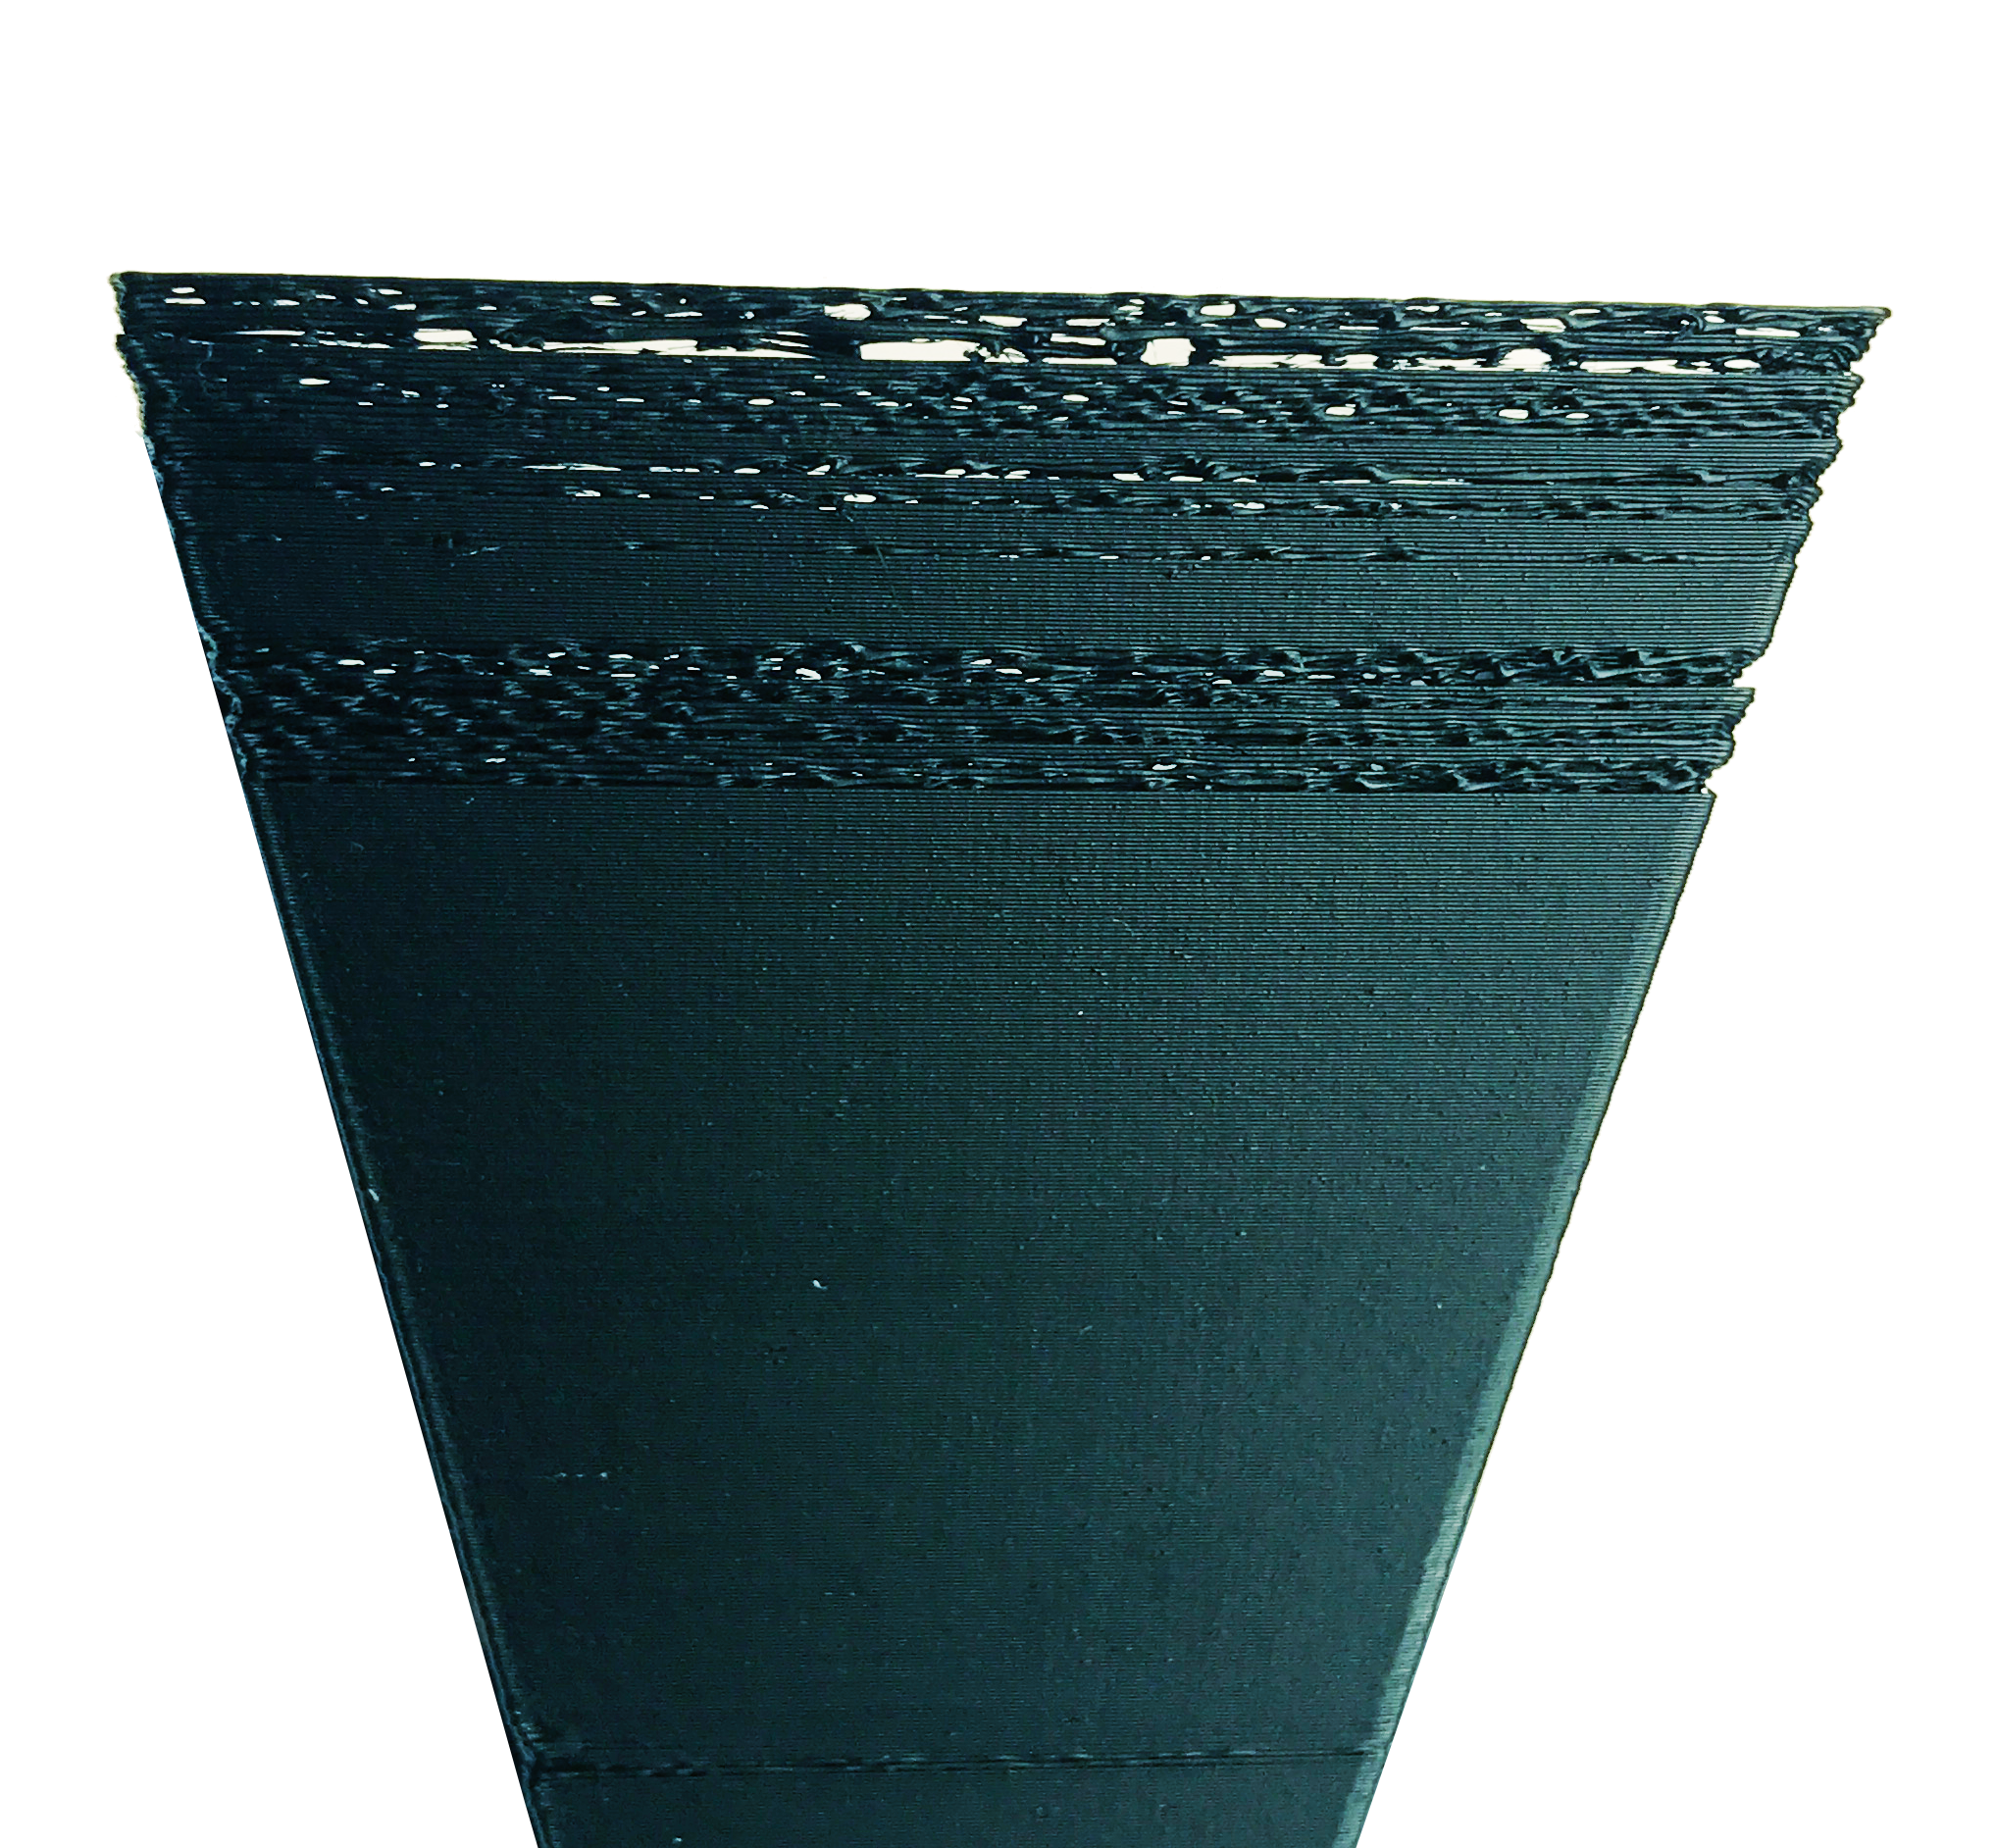
\includegraphics[width=9.5cm]{pics/HornFail}
\caption{Důsledek ucpavání trysky v průběhu tisku modelu}
\label{fig:HornFail}
\end{center}
\end{figure}


\subsubsection{Anténní čočka}
Realizace anténní čočky je v porovnání s předchozím případem velmi zjednodušena z důvodu zvolení zpomalujícího typu, tedy použití dielektrického, nikoliv vodivého, materiálu.

Pro správnou funkci čočky a maximálnímu přiblížení se simulovaných modelů je důležité při generování dat pro technologický proces použít správný typ vnitřní struktury pro zajištění 100\.\% podílu dielektrického materiálu.

Pokud toto nebude při realizaci dodrženo, vlivem nehomogenního prostředí pro šíření vlny, obsahující mnoho velmi ostrých rozhraní vzduch/dielektrikum, způsobí velmi odlišné chování a pro jeho dostatečný popis je třeba k téro struktuře přistupovat jako k metamateriálu.


\section{Pokovení}
Jelikož již dostupné vodivé filamenty disponují velmi malou vodivostí pro přímé použití, pro možnost následného pokovení však mohou být více než dostačující.

\subsubsection{Mokrá cesta}
Jako první cesta pro maximalizaci vodivosti produktu byla zvolena metoda elektricky vodivého laku EMI 35\cite{EMIdata}.

Použitý elektrický lak je založen na termoplastickém polymeru s přidaným speciálním měděným pigmentem rozpuštěném ve vhodné ředící složce. Po aplikaci laku v průběhu 24 hodin dojde k postupnému odpaření ředící složky a vznikne tenká vodivá vrstva, o tloušťce v řádu 50\,$\mu$m.

Při zvolení této cesty není nutno realizovat strukturu z vodivého polymeru jelikož přilnutí vodivé látky není podmíněno jeho vodivostí.


\begin{figure}[h]
\begin{center}
%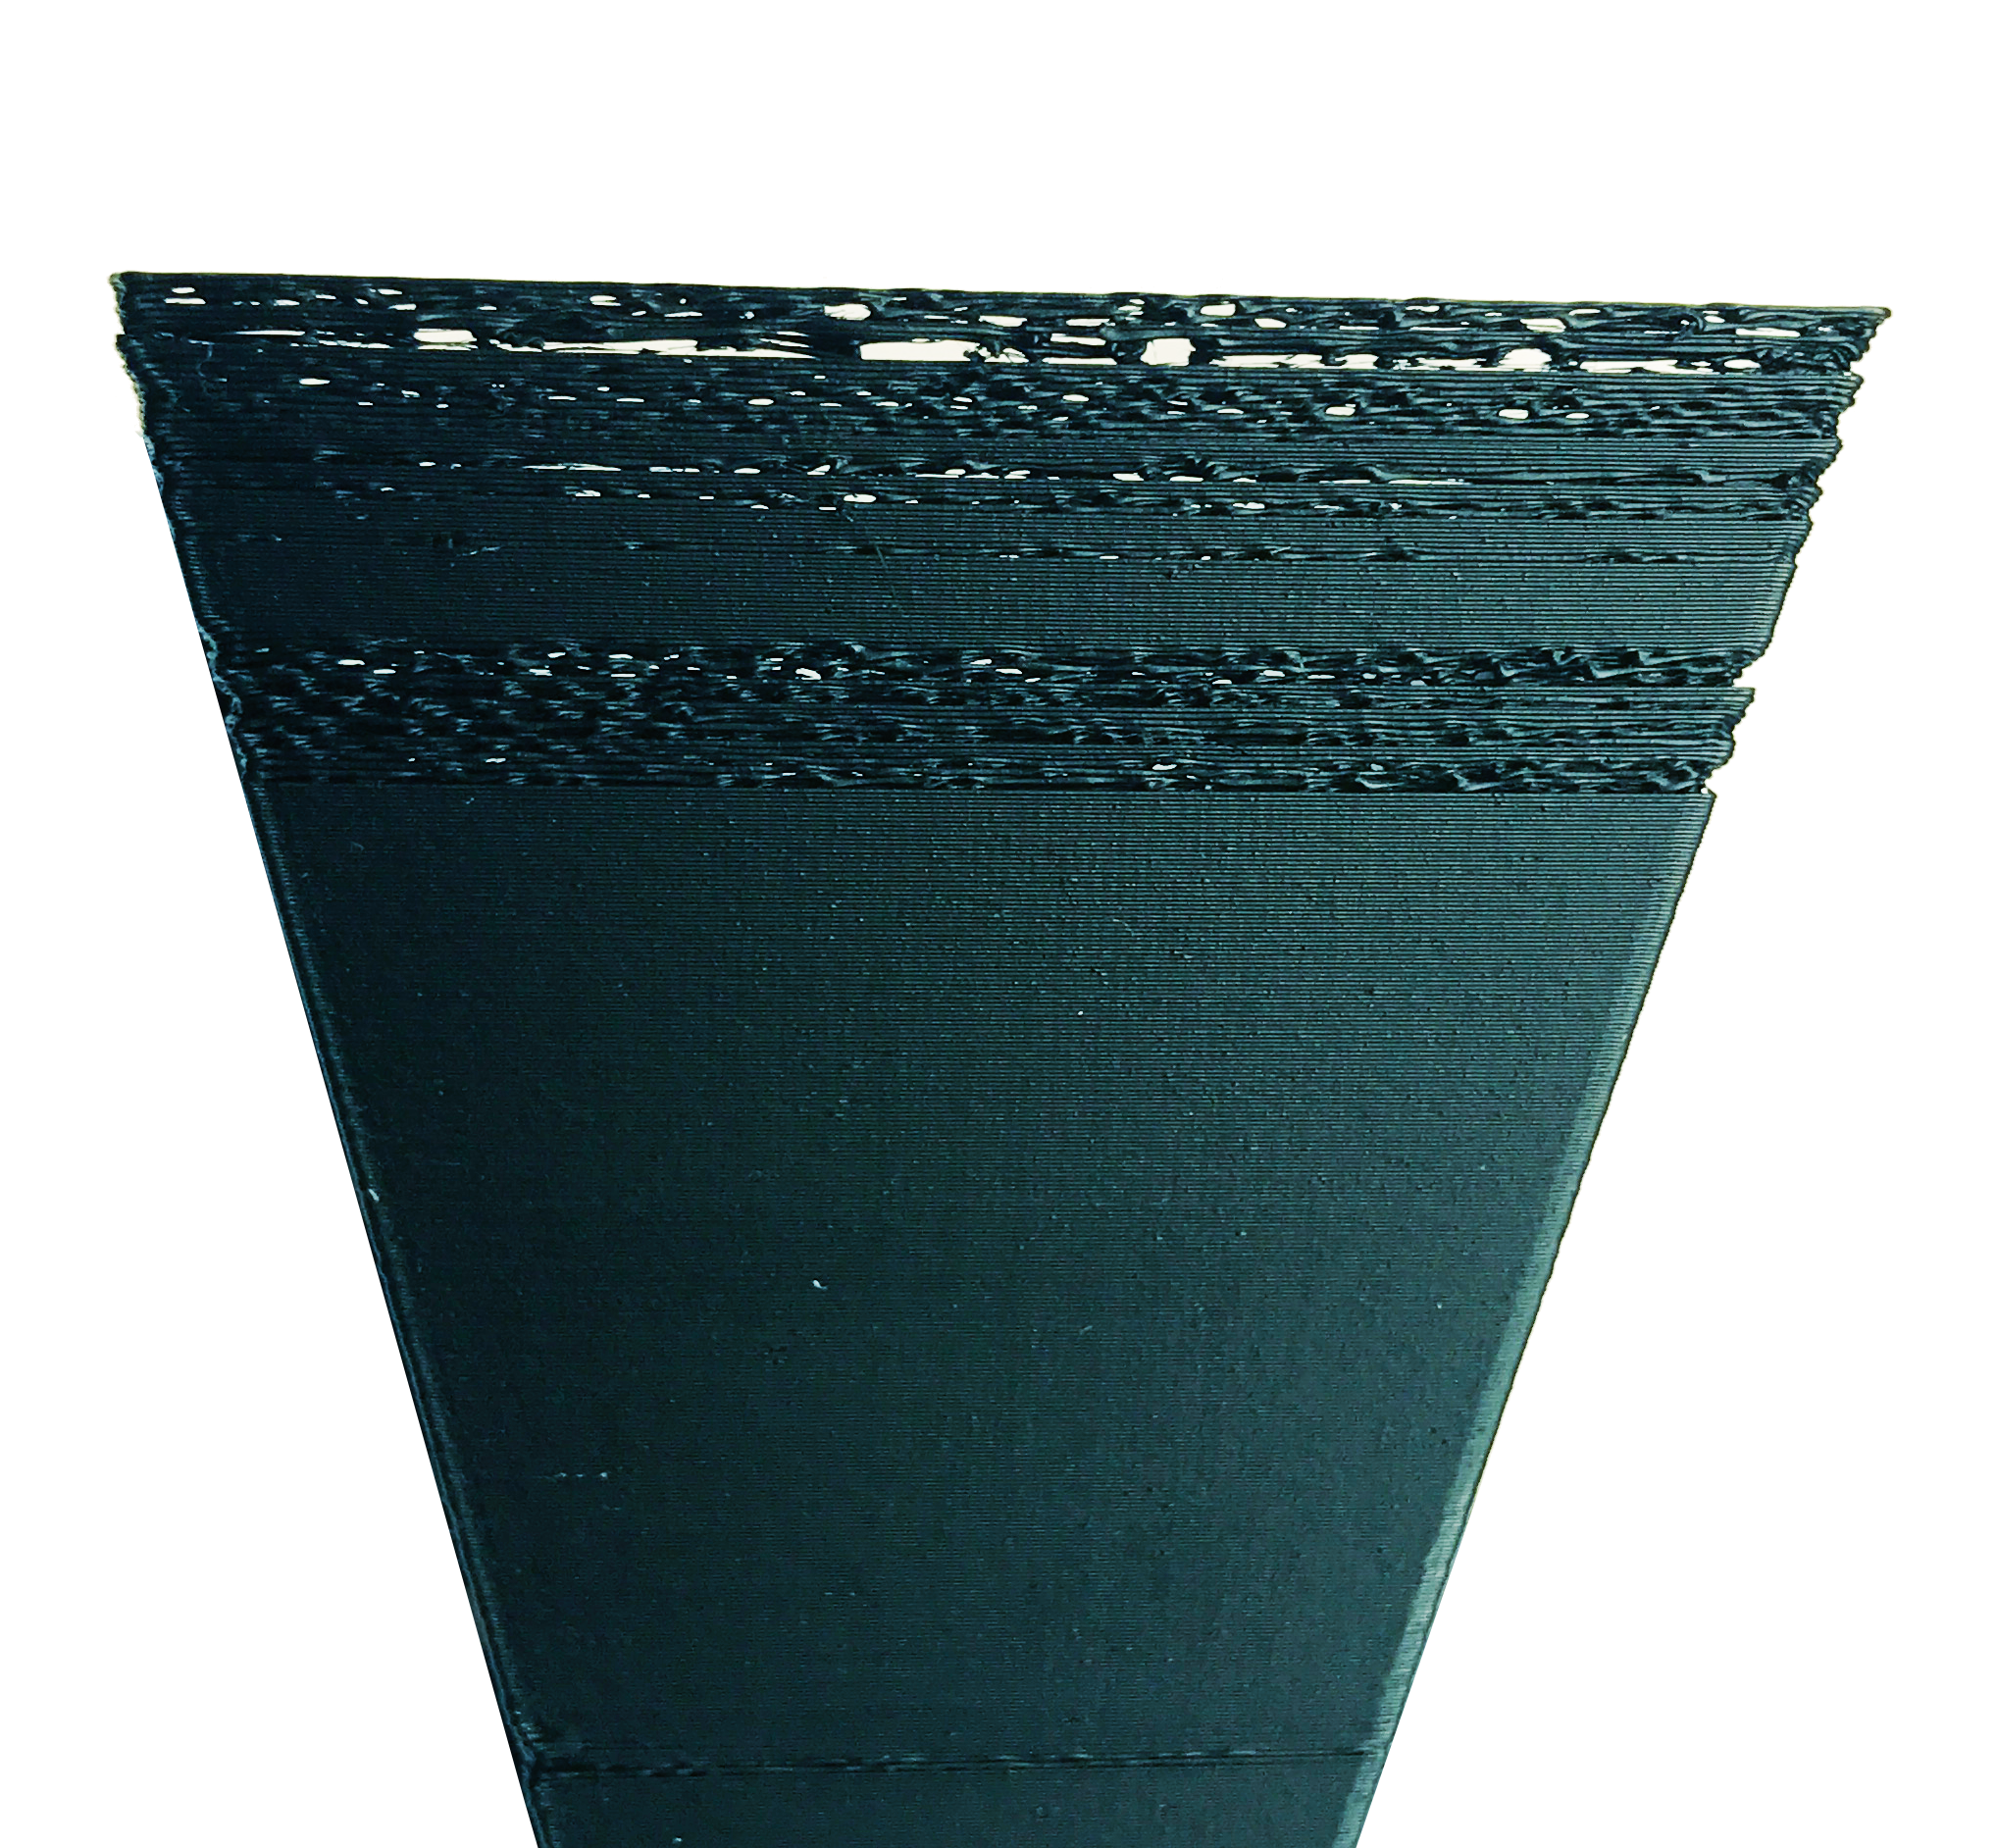
\includegraphics[width=9.5cm]{pics/HornFail}
\caption{Realizovaná struktura s následným nánosem EMI 25}
\label{fig:HornEMI}
\end{center}
\end{figure}

\subsubsection{Elektroformování}
Galvanoplastika je technologie známá a využívaná po mnoho desítek let. Jejím principem je elektroformování (z anglického „electroforming“) geometrických tvarů s využitím elektrochemického vylučování kovových povlaků na primární model. Využívá se principu elektrolýzy, avšak vylučovány jsou vrstvy v od desítek mikrometrů po jednotky milimetrů.\cite{Electroforming}.

Jelikož tato metoda je závislá na principu elektrolýzy, je nutné aby pokovovaný objekt vykazoval dostatečnou vodivost právě pro zajištění nutných podmínek vzniku. Toto může být například realizování například EMI 25 lakem, které mají však svá omezení. Pokud však vstupní vzorek již vykazuje vyšší vodivost, velmi se proces zjednoduší a není třeba využívat komplexních způsobů "zvodivení".

Pokud tedy realizujeme strukturu například z filamentu F-electric, který při prvních testech byl stoprocentně úspěšný, můžeme ji následně přímo pokovit elektroformováním.

Tento postup byl nejprve otestován v laboratorních podmínkách při prvotním testování před započatím této práce. Při výzkumu možností byla navržena základní mřížková struktura pro ověření použitelnosti metody. Dále pak bylo pozorováno velmi gradientní rozložení elektrického potenciálu, které řetězovou reakcí způsobylo nekonzistentní výsledné vrstvy s maximem u přípojného bodu elektrody.

Pro kompenzaci tohoto gradientního rozložení pole je možno využít postupné noření do lázně smeřem k přípojnému bodu za správné rychlosti.
\begin{figure}[h]
\begin{center}
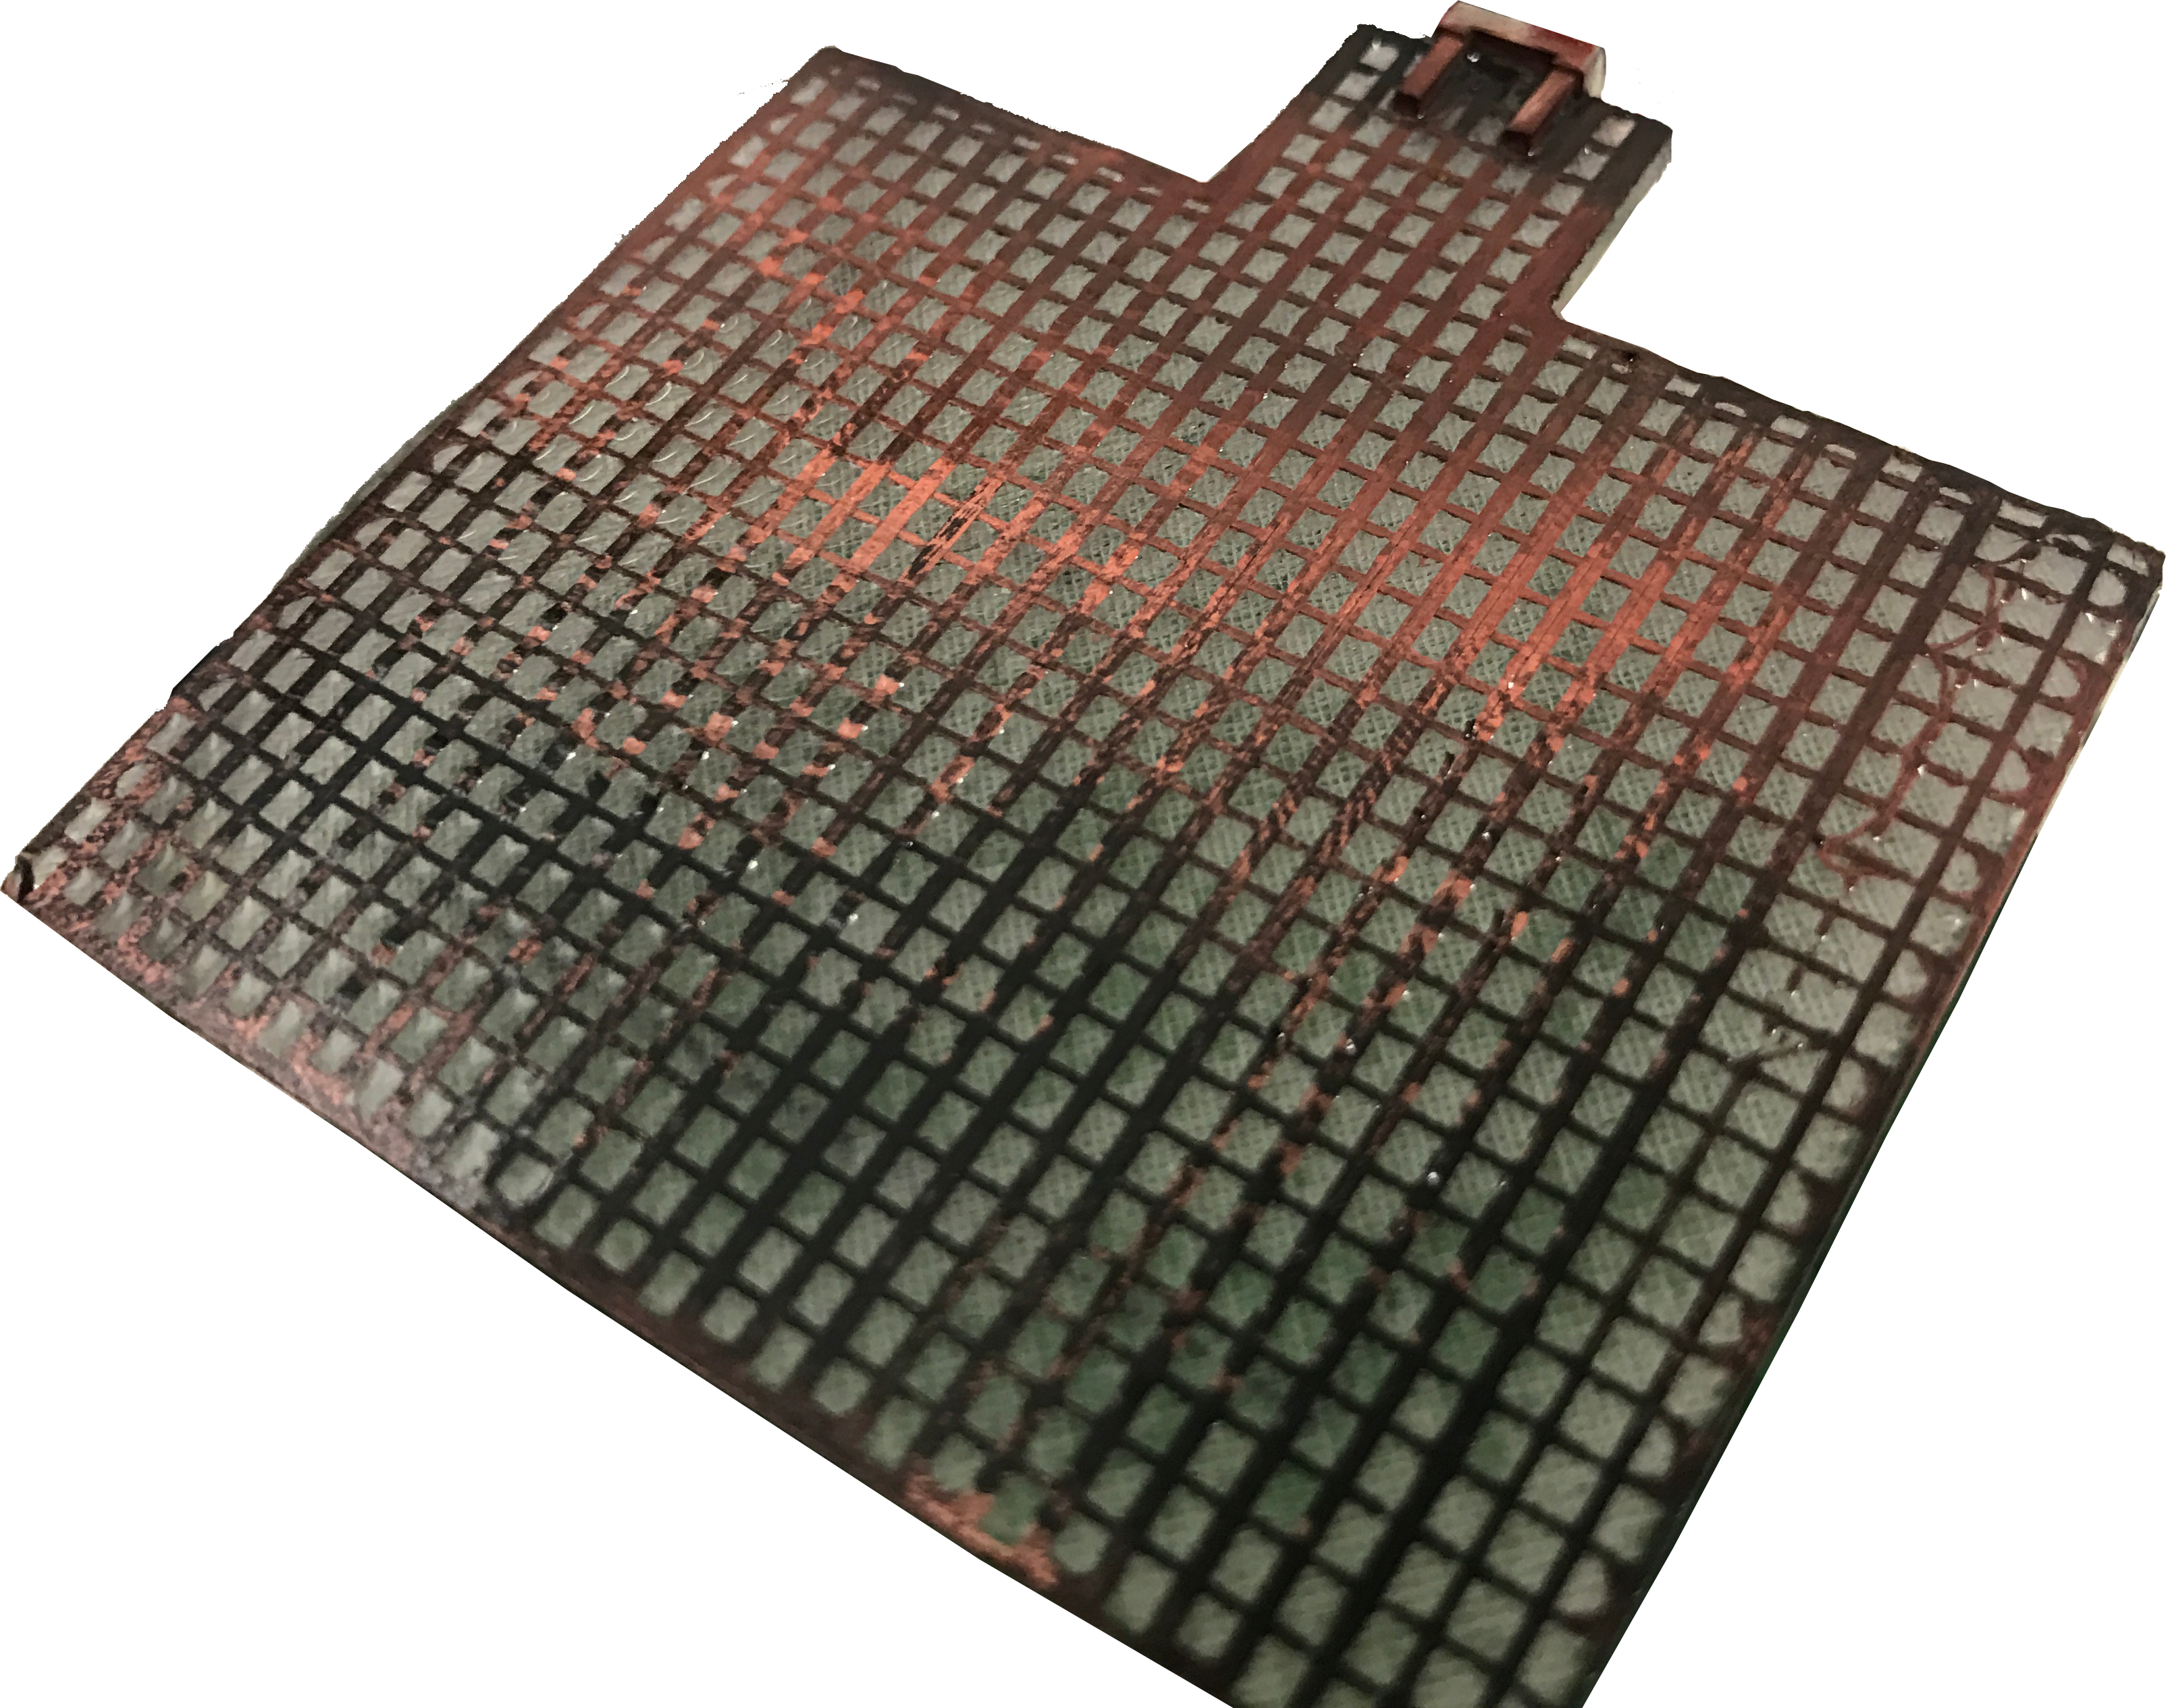
\includegraphics[width=9.5cm]{pics/platingtest}
\caption{Výsledná testovací struktura s výraně viditělnou nekonzistentní vrstvou}
\label{fig:platingtest}
\end{center}
\end{figure}

Z důvodu toho, že se tento postup jevil jako velmi perspektivní, byla navázána spolupráce se společností Electroforming s.r.o. pro možnost využití produkčních zařízení za účelem pokovení realizované trychtýřové antény z materiálu F-electric.

Výsledkem této spolupráce byl velmi pozitivní z hlediska kvality a přilnavosti nanešené vrstvy (pomineme-li popsaná omezení technologie v 3.1 a přilnavost na hladké povrchy) a její vodivosti. Výsledná struktura při testu ohmického odporu standartním multimetrem CEM DT-61 vykazovala hodnoty pod rozlišovací schopnost.

Nicméně však vzhledem ke komunikačnímu šumu ve spolupráci, a nepředáním vzájemných znalostí pužitých technologíí došlo k deformaci výsledné struktury. Jelikož materiál použitý pro realizaci struktury disponuje teplotou skelného přechodu $\vartheta_g \simeq 50\,^\circ$$C$ a teploty lázní procesu pokovení tuto teplotu standartně přesahují. Na základě této zkušenosti byla varžena speciálně modifikovaná struktura, viz 3.1, bohužel však vlivem výše uvedených komplikací se ji již nepodařilo realizovat, to ale nevylučuje realizovatelnost, jen vyžaduje delší výzkum samotných materiálů.


\begin{figure}[h]
\begin{center}
\includegraphics[width=9.5cm]{pics/plated/deform}
\caption{Deformace a nedokonalosti v dutině výsledné pokovené struktury}
\label{fig:PLdef}
\end{center}
\end{figure}

\begin{figure}[h]
\begin{center}
\includegraphics[width=9.5cm]{pics/plated/adhes}
\caption{Nízká přilnavost k hladkým povrchům}
\label{fig:PLadh}
\end{center}
\end{figure}


\section{Měření parametrů}

\begin{figure}
\begin{tikzpicture}[scale=1.4]
\begin{axis}[
    xlabel={Angle /\,$^\circ$},
    ylabel={Amplitude /\,dB},
    minor tick num=10,
    minor grid style={gray!25},
  	major grid style={black!50},
  	xmin=-180,xmax = 180,
  	ymin=-120, ymax=-60,
    grid=both
]
\addplot [no markers, thick, blue] table [col sep=tab, y=Ae-graph] {horn.dat};
\addplot [no markers, thick, red] table [col sep=tab, y=Ae-emi] {horn.dat};
\addplot [no markers, thick, green] table [col sep=tab, y=Ae-lens] {horn.dat};
\end{axis}
\end{tikzpicture}
\caption{Řez naměřené vyzařovací charakteristiky realizovaného trychtýře z materiálu F-electric v E rovině}
\end{figure}

\begin{figure}
\begin{tikzpicture}
\begin{axis}[
    xlabel={Angle /\,$^\circ$},
    ylabel={Amplitude /\,dB},
    minor tick num=10,
    minor grid style={gray!25},
  	major grid style={black!50},
  	xmin=-180,xmax = 180,
  	ymin=-120, ymax=-60,
    grid=both
]
\addplot [no markers, thick, blue] table [col sep=tab, y=Ah-graph] {horn.dat};
\addplot [no markers, thick, red] table [col sep=tab, y=Ah-emi] {horn.dat};
\addplot [no markers, thick, green] table [col sep=tab, y=Ah-lens] {horn.dat};
\end{axis}
\end{tikzpicture}
\caption{Řez vyzařovací charakteristiky v H rovině}
\end{figure}




%% This is an example first chapter.  You should put chapter/appendix that you
%% write into a separate file, and add a line \include{yourfilename} to
%% main.tex, where `yourfilename.tex' is the name of the chapter/appendix file.
%% You can process specific files by typing their names in at the 
%% \files=
%% prompt when you run the file main.tex through LaTeX.
\chapter{Závěr}
Cílem této diplomové práce bylo realizovat trychtýřovou anténu s dielektrickou čočkou technologií 3D tisku s hlavním zaměřením na optimalizace struktur vyhovujících právě použité technologii. 

Struktury byly úspěšně realizovány jak z vodivých, tak standartních termoplastických polymerů, včetně čočky. Funkčnost vytvořených struktur byla ověřena měřením.

Na základě změřených směrových charakteristik (obrázek \ref{fig:FarfieldsE}, \ref{fig:FarfieldsH}) a jejich výsledků nebylo relevantní pokračovat v měření zisku realizovaných struktur vlivem velmi malého přijatého výkonu, což je způsobeno velkými ztrátami na strukturách (jak F-electric "vodivého" filamentu, tak při následném pokovení EMI 35).

Pro zlepšení parametrů, bylo předvedeno i řešení s možným následným pokovením, kde byla projevena velká iniciativa ze strany společnosti Electroforming s.r.o. na základě předvedených vzorků realizovaných elektricky vodivým materiálem, zejména z důvodu možného vypuštění nebezpečných procesů, které je nutno podstupovat při použití standartních polymerních materiálů. Bohužel se však toto řešení nepodařilo zdárně realizovat z důvodu vysokých teplot při procesu což způsobilo deformaci struktury, viz obrázek \ref{fig:PLdef}. Galvanizační lázeň lze ale optimalizovat pro provoz při nižších teplotách.

Dále se naskýtají možnosti využití v tisku ryze dielektrických struktur, jako například rezonátorů. Je tedy velká motivace rozvíjet dále možnosti aplikace této technologie, jelikož má velký potenciál pro tisk materiálů s vnitřními strukturami oproti ostatním technologiím, dále je třeba nezapomenout že vodivé materiály, které byly v této práci použity, jsou jedny z prvních dostupných a stále probíhá vývoj s cílem přiblížení se ideálním parametrům.



%
\begin{thebibliography}{9}

\bibitem{ModernLens}
  John Thornton,
  Kao-Cheng Huang,
  MODERN LENS ANTENNAS FOR COMMUNICATIONS ENGINEERING,
  Wiley,
  IEEE PRESS,
  2013.

\bibitem{Dolecek}
  Josef Doleček,
  Fillamentum,
  Parzlich s.r.o.,
  Konzultace na téma výroby filamentů,
  2016.

\bibitem{ConstantineTheory}
  Constantine A. Balanis,
  Antenna theory analysis and design,
  Wiley,
  4th edition,
  2016.

\bibitem{3Dhubs}
  https://www.3dhubs.com/trends,
  2017.
  

\end{thebibliography}

\newpage

\listoffigures

\newpage

\listoftables

%% $Log: abstract.tex,v $
% Revision 1.1  93/05/14  14:56:25  starflt
% Initial revision
% 
% Revision 1.1  90/05/04  10:41:01  lwvanels
% Initial revision
% 
%
%% The text of your abstract and nothing else (other than comments) goes here.
%% It will be single-spaced and the rest of the text that is supposed to go on
%% the abstract page will be generated by the abstractpage environment.  This
%% file should be \input (not \include 'd) from cover.tex.
\thispagestyle{empty}
\chapter*{Seznam použitých symbolů a zkratek}
\thispagestyle{empty}
\itab{3D} \tab{} \tab{3-rozměrné}\\*
\itab{LED} \tab{} \tab{Světlo emitující dioda}\\*
\itab{CD} \tab{} \tab{Kompaktní disk}\\*
\itab{VNA} \tab{} \tab{Vector network analyzer}\\*
\itab{ABS} \tab{} \tab{Acrylonitrile butadiene styrene}\\*
\itab{PLA} \tab{} \tab{Polylactic acid}\\*
\itab{PET} \tab{} \tab{Polyethylene terephthalate}\\*
\itab{D.U.T.} \tab{} \tab{Device under test}\\*


%\include{99-add-safety}
%
\chapter{Obsah přiloženého CD}
Na přiloženém CD jsou uloženy v adresáři:
\begin{itemize}
\item \textbf{man-data} všechna výrobní data použita při řešení práce.
\item \textbf{text} je uložena tato práce ve formátu *.pdf.
\end{itemize} 


\thispagestyle{empty}
\null\newpage

%%\include{biblio}
\end{document}

